\documentclass[10pt]{article}

% ---------------------------------------------------------------------------
% Packages (all in a standard TeX Live install)
% ---------------------------------------------------------------------------
\usepackage[utf8]{inputenc}
\usepackage[T1]{fontenc}
\usepackage[margin=1in]{geometry}
\usepackage{amsmath,amssymb}
\usepackage{booktabs}
\usepackage{graphicx}
\usepackage{xcolor}
\usepackage{caption}
\usepackage{subcaption}
\usepackage{listings}
\usepackage{pgfplots}
\pgfplotsset{compat=1.17}
\usetikzlibrary{positioning,arrows.meta,fit,backgrounds,shapes.geometric,calc}
\usepackage[hidelinks]{hyperref}
\usepackage{bookmark}   % stable PDF outlines without an extra pdflatex pass
\usepackage{url}

% ---------------------------------------------------------------------------
% Listings style for code / config snippets
% ---------------------------------------------------------------------------
\definecolor{codebg}{RGB}{247,247,247}
\definecolor{codekw}{RGB}{0,90,160}
\definecolor{codecm}{RGB}{110,110,110}
\lstset{
  basicstyle=\ttfamily\small,
  backgroundcolor=\color{codebg},
  keywordstyle=\color{codekw}\bfseries,
  commentstyle=\color{codecm}\itshape,
  breaklines=true,
  frame=single,
  framesep=4pt,
  rulecolor=\color{gray!40},
  showstringspaces=false,
  captionpos=b,
}

\newcommand{\filesmin}{files\,min\textsuperscript{-1}}
\newcommand{\rtf}{$\times$RT}
\newcommand{\msd}[2]{$#1\,(#2)$}

% ---------------------------------------------------------------------------
\title{\textbf{Throughput Scaling of a GPU Speech Transcription and\\
Diarization Service: Threads Fail, Processes Win, and a\\
Gateway Ties Them Together}}

\author{%
  Gregorio Toscano\thanks{Corresponding author.}\\
  The Catholic University of America\\
  \texttt{toscanopulido@cua.edu}
  \and
  Grace Connors\\
  The Catholic University of America\\
  \texttt{connorsg@cua.edu}
}
\date{\today}

% ---------------------------------------------------------------------------
\begin{document}
\maketitle

\begin{abstract}
Speaker-attributed speech transcription combines automatic speech recognition
(ASR), forced alignment, and speaker diarization into a single pipeline. Such
pipelines are widely deployed as GPU services, yet their concurrency behaviour
is poorly characterised: practitioners routinely assume that a GPU-resident
model is GPU-bound and that adding worker threads will raise throughput. We show
this assumption is wrong for the popular \emph{WhisperX} pipeline (Whisper
\texttt{large-v3} + wav2vec2 alignment + pyannote diarization). Through
controlled measurements on an NVIDIA RTX PRO 6000 GPU we find that (i) a single
transcription stream leaves the GPU only $40$--$44\%$ utilised because
alignment and diarization are CPU- and Python-bound, (ii) allowing a second
worker \emph{thread} to run concurrently within one process \emph{reduces}
throughput by $28\%$ due
to contention on the CPython Global Interpreter Lock (GIL) and the GPU, while
(iii) replicating the service as independent \emph{processes} yields near-ideal
speedup initially, followed by diminishing returns ($1.50\times$ at three
replicas for the short workload and $1.70\times$ at four for the long workload;
$73$--$81\%$ utilisation). We then introduce a lightweight nginx
\emph{gateway} that presents a single endpoint and round-robins requests across
replicas; because each replica's job registry is process-local, we route job
status requests back to the owning replica by encoding the replica identity in
the job identifier. Across five trials, the gateway shows no throughput penalty:
its mean is $1$--$2\%$ above direct routing, within the observed execution
variability. Finally we give a remainder-aware wave model for the wall-clock
time of a batch of $N$ files on $R$ replicas. Three end-to-end trials show that
the synchronized-wave estimate is conservative for continuously queued work,
overpredicting the mean wall time by $4$--$7\%$. Our
results give practitioners a concrete recipe for sizing single-GPU speech
services and a cautionary tale about thread-level parallelism in GIL-bound
GPU pipelines.
\end{abstract}

% ===========================================================================
\section{Introduction}
\label{sec:intro}

Automatic transcription of long-form, multi-speaker audio---meetings, hearings,
interviews, podcasts---has become a commodity workload, driven by the accuracy
of the Whisper family of models~\cite{radford2023whisper} and by open pipelines
such as WhisperX~\cite{bain2023whisperx} that add word-level timestamps and
speaker labels. A common deployment pattern is a GPU-resident service: a
long-running process that loads the models once and serves transcription
requests over HTTP.

When such a service must handle several recordings concurrently, the operator
faces a sizing question: \emph{how many simultaneous transcriptions can one GPU
sustain, and what wall-clock time should a batch of $N$ files take?} The folk
answer is that a GPU model is GPU-bound, so one should raise an intra-process
worker count until the GPU saturates. We show that this reasoning fails for
speaker-attributed transcription, for two compounding reasons. First, only part
of the pipeline runs on the GPU: forced alignment and, especially, neural
speaker diarization spend substantial time in Python and on the CPU, so a single
stream leaves the GPU well under half utilised. Second, because that work runs
in Python, additional \emph{threads} cannot execute it in parallel---the CPython
Global Interpreter Lock (GIL)~\cite{cpythongil} serialises Python bytecode---so
thread-level workers contend on the GIL and on the GPU and make throughput
\emph{worse}.

We make the following contributions:
\begin{itemize}
  \item A measurement study (\S\ref{sec:results}) quantifying the GIL/CPU
  bottleneck in the WhisperX pipeline and showing that thread-level parallelism
  regresses throughput while process-level replication scales it.
  \item A single-GPU replica architecture with an nginx gateway
  (\S\ref{sec:arch}) that gives clients one endpoint. We identify and solve the
  \emph{process-local job registry} problem by encoding replica identity in the
  job identifier and routing status requests accordingly.
  \item An evaluated, remainder-aware wave model (\S\ref{sec:model}) that
  conservatively estimates homogeneous batch completion time from
  concurrency-specific service times.
\end{itemize}

All experiments use a single GPU and off-the-shelf components; our aim is a
reproducible recipe rather than a new model or kernel. The complete
implementation---service, multi-GPU launcher, gateway, and benchmark suite---is
open source.\footnote{\url{https://github.com/gtoscano/Parascribe}}

% ===========================================================================
\section{Background}
\label{sec:background}

\paragraph{The WhisperX pipeline.}
For each request the service runs four stages:
(1) \emph{ASR}: Whisper \texttt{large-v3}~\cite{radford2023whisper} executed
through faster-whisper~\cite{fasterwhisper} / CTranslate2~\cite{ctranslate2},
producing text with coarse segment timestamps;
(2) \emph{alignment}: a wav2vec2 phoneme model~\cite{baevski2020wav2vec2} forces
word-level timestamps;
(3) \emph{diarization}: the pyannote \texttt{speaker-diarization-3.1}
pipeline~\cite{bredin2020pyannote,bredin2023pyannote,plaquet2023powerset}
segments the audio by speaker;
(4) \emph{assignment}: words are attributed to speakers and relabelled.
Stages~1 and~2 are dominated by GPU tensor operations, but stage~3 performs
significant CPU-side clustering and stages~2--4 involve substantial Python-level
orchestration.

\paragraph{The GIL.}
CPython executes at most one thread of Python bytecode at a time, guarded by the
GIL~\cite{cpythongil}. Native extensions (PyTorch kernels, CTranslate2) release
the GIL while running C++/CUDA code, so a single Python thread \emph{can} keep
the GPU busy. However, any pipeline phase that stays in Python---graph
manipulation, clustering bookkeeping, segment assignment, audio I/O---holds the
GIL, and two Python threads cannot run those phases simultaneously.

\paragraph{Thread-safety.}
An orthogonal constraint: the pyannote~3.x diarization pipeline is not
thread-safe, so a shared model instance cannot be driven from multiple threads
regardless of the GIL. Any concurrency scheme must therefore give each worker
its own diarization model.

% ===========================================================================
\section{System Architecture}
\label{sec:arch}

\subsection{Baseline service}
The service is a FastAPI/Uvicorn application in a Docker container. It exposes an
asynchronous submit endpoint that enqueues a job and returns a job identifier,
plus polling endpoints for status and results. A configurable number of worker
tasks (\texttt{WORKERS}) drain the queue; each worker owns a private
\emph{model set} (ASR, per-language alignment, diarization) so that diarization
is never shared across threads. Results are also written to a shared volume as
files, so completed transcripts survive process restarts.

\subsection{Thread-level parallelism (the tempting wrong answer)}
Setting $\texttt{WORKERS}>1$ spawns multiple worker threads in the one process,
each with its own model set, and runs each job's blocking pipeline in a thread
pool. This is the natural first attempt at concurrency. \S\ref{sec:results}
shows it does not work: the Python-bound phases serialise on the GIL and the
threads additionally contend for the GPU.

\subsection{Process-level replication}
Real parallelism requires separate interpreters. We run $R$ identical container
\emph{replicas} of the service, each with $\texttt{WORKERS}=1$, all pinned to the
same GPU. Each replica has its own Python process (own GIL) and its own CUDA
context, so up to $R$ jobs execute genuinely concurrently, bounded only by GPU
compute and memory. On our hardware a replica's resident footprint is
$\approx 13$\,GB, so memory is not the binding constraint on a $96$\,GB GPU;
compute is.

\subsection{The gateway and the process-local registry problem}
\label{sec:gateway}
Exposing $R$ replicas to clients as $R$ URLs pushes load-balancing into every
client. We instead front the replicas with an nginx gateway that presents a
single endpoint and round-robins requests (Figure~\ref{fig:arch}). One subtlety
makes a na\"ive proxy incorrect: each replica's job registry is \emph{in-memory and process-local}. A
job submitted to replica~$A$ is unknown to replica~$B$, so a status poll that a
plain round-robin proxy sends to $B$ returns \texttt{404}.

We solve this without shared state by encoding the owning replica in the job
identifier. Replica~$i$ mints identifiers of the form \texttt{i-\{token\}}. The
gateway round-robins only the submit endpoint; for job-scoped requests it
extracts the numeric prefix and routes to that replica
(Listing~\ref{lst:nginx}). Because the transcript files are also written to a
shared volume, results remain retrievable even across restarts.

\begin{figure}[t]
\centering
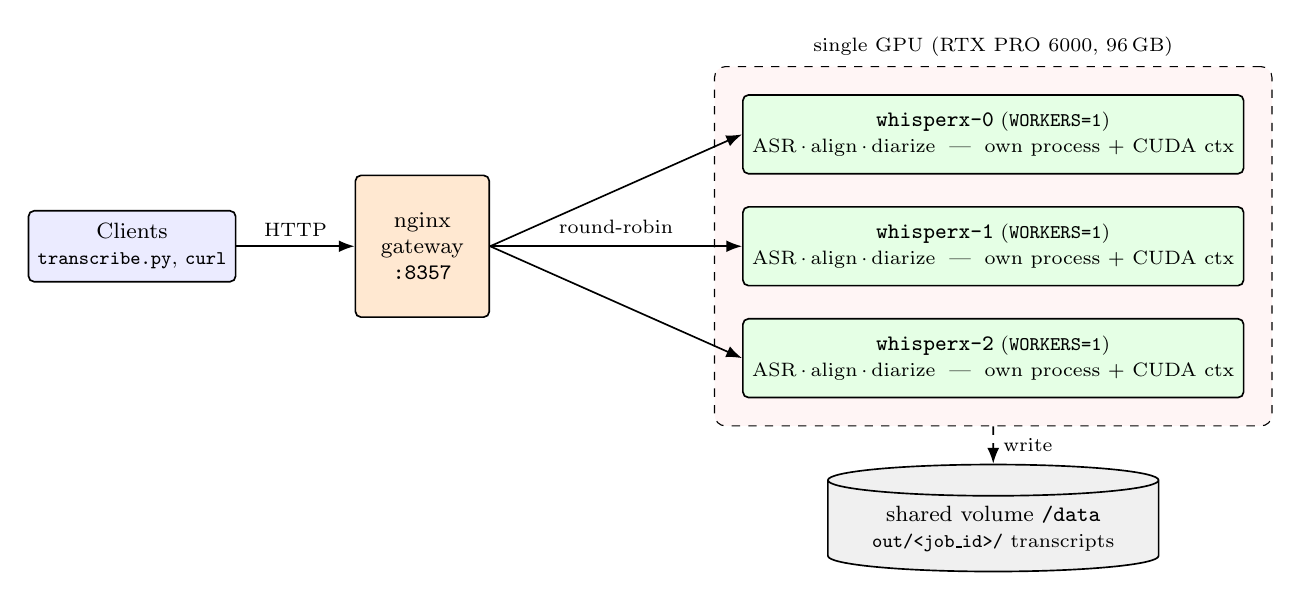
\begin{tikzpicture}[
  font=\footnotesize, >=Latex,
  comp/.style={draw, semithick, rounded corners=2pt, align=center,
               minimum height=9mm},
  client/.style={comp, fill=blue!8, minimum width=22mm},
  gw/.style={comp, fill=orange!18, minimum width=17mm, minimum height=18mm},
  rep/.style={comp, fill=green!10, minimum width=45mm, minimum height=10mm},
  vol/.style={draw, semithick, cylinder, shape border rotate=90, aspect=0.12,
              fill=gray!12, align=center, minimum width=42mm, minimum height=7mm},
  flow/.style={->, semithick},
]
% clients and gateway
\node[client] (cli) {Clients\\{\scriptsize\texttt{transcribe.py}, \texttt{curl}}};
\node[gw, right=15mm of cli] (gw) {nginx\\gateway\\\texttt{:8357}};
% replicas (r1 level with gateway, r0 above, r2 below)
\node[rep, right=32mm of gw] (r1)
  {\texttt{whisperx-1}\;{\scriptsize(\texttt{WORKERS=1})}\\%
   {\scriptsize ASR\,$\cdot$\,align\,$\cdot$\,diarize \;|\; own process + CUDA ctx}};
\node[rep, above=4mm of r1] (r0)
  {\texttt{whisperx-0}\;{\scriptsize(\texttt{WORKERS=1})}\\%
   {\scriptsize ASR\,$\cdot$\,align\,$\cdot$\,diarize \;|\; own process + CUDA ctx}};
\node[rep, below=4mm of r1] (r2)
  {\texttt{whisperx-2}\;{\scriptsize(\texttt{WORKERS=1})}\\%
   {\scriptsize ASR\,$\cdot$\,align\,$\cdot$\,diarize \;|\; own process + CUDA ctx}};
% GPU backdrop around the replicas
\begin{scope}[on background layer]
  \node[draw, dashed, rounded corners, fill=red!4, inner sep=3.5mm,
        fit=(r0)(r2),
        label={[font=\scriptsize]above:single GPU (RTX PRO 6000, 96\,GB)}]
        (gpu) {};
\end{scope}
% shared volume below the GPU
\node[vol] (vol) at ($(gpu.south)+(0,-13mm)$)
  {shared volume \texttt{/data}\\{\scriptsize \texttt{out/<job\_id>/} transcripts}};
% flows
\draw[flow] (cli) -- node[above,font=\scriptsize]{HTTP} (gw);
\draw[flow] (gw.east) -- node[above=1pt,font=\scriptsize,pos=0.5]{round-robin} (r1.west);
\draw[flow] (gw.east) -- (r0.west);
\draw[flow] (gw.east) -- (r2.west);
\draw[flow,dashed] (gpu.south) -- node[right,font=\scriptsize]{write} (vol.north);
\end{tikzpicture}
\caption{System architecture. Clients issue HTTP to a single nginx gateway
(\texttt{:8357}). The gateway round-robins \texttt{POST /v1/transcribe} across the
$R$ process replicas and routes each \texttt{GET /v1/jobs/}\textit{i}\texttt{-\dots}
back to the owning replica~\textit{i} by the numeric job-id prefix, so the
process-local job registries need no shared state. Each replica is an independent
OS process---its own Python interpreter (hence its own GIL) and CUDA
context---running \texttt{WORKERS=1} with a private ASR/align/diarize model set;
all $R$ replicas share one GPU. Finished transcripts are written to a shared
\texttt{/data} volume.}
\label{fig:arch}
\end{figure}

\begin{lstlisting}[language=,caption={nginx routing: round-robin submits,
prefix-route job lookups.},label={lst:nginx},captionpos=b]
resolver 127.0.0.11;                 # Docker embedded DNS
upstream pool { server r0:8000; server r1:8000; server r2:8000; }

# Job status/results -> the replica named in the id prefix
location ~ ^/v1/jobs/(?<rid>[0-9]+)- {
    set $backend r$rid:8000;
    proxy_pass http://$backend;
}
# Submit + health + models -> round-robin the pool
location / { proxy_pass http://pool; }
\end{lstlisting}

Two operational notes proved important in practice: a single nginx worker
process is preferable because per-worker round-robin counters otherwise skew the
distribution on small samples; and the gateway must wait for replicas to become
healthy before serving, or its failover logic transiently concentrates load on
the first ready replica.

% ===========================================================================
\section{Experimental Setup}
\label{sec:setup}

\paragraph{Hardware.} A workstation with two NVIDIA RTX PRO 6000 (Blackwell)
GPUs, $97\,887$\,MiB ($\approx 96$\,GiB) each. The transcription service is
pinned to one GPU; the other hosts an unrelated model and is not used by our
experiments.

\paragraph{Software.} Whisper \texttt{large-v3} via
faster-whisper~\cite{fasterwhisper}\,/\,CTranslate2~4.8.0~\cite{ctranslate2},
float16, batch size~16; wav2vec2 English
alignment~\cite{baevski2020wav2vec2}; the pyannote
\texttt{speaker-diarization-3.1}
pipeline~\cite{bredin2023pyannote,plaquet2023powerset} on
PyTorch~\cite{paszke2019pytorch}; FastAPI + Uvicorn; Docker with the NVIDIA
runtime; nginx (Alpine) as the gateway.

\paragraph{Workloads.} Two representative recordings
(Table~\ref{tab:workloads}): a short 8-minute meeting excerpt (AMI
corpus~\cite{carletta2005ami}, 4 speakers) and a long 40-minute oral argument
(Oyez, 8 speakers). The short workload isolates per-request overheads and lets
us sweep concurrency cheaply; the long workload reflects realistic batch jobs.

\begin{table}[t]
\centering
\caption{Workloads.}
\label{tab:workloads}
\begin{tabular}{lccc}
\toprule
Tag & Source & Duration & Speakers \\
\midrule
W-short & AMI meeting & $477.9$\,s ($\approx 8$\,min) & 4 \\
W-long  & Oyez argument & $2400$\,s ($40$\,min) & 8 \\
\bottomrule
\end{tabular}
\end{table}

\paragraph{Methodology.} A load generator submits $c$ identical jobs
concurrently and records: wall-clock time for the batch; per-job service time
(server-side running$\rightarrow$finished); GPU memory, utilisation and power
draw sampled at 2\,Hz via \texttt{nvidia-smi}; host RAM; and host CPU occupancy
derived from \path{/proc/stat} deltas. CPU is reported in \emph{cores busy}
rather than a percentage, since a percentage is not actionable for provisioning
without the core count. Per-replica CPU and resident set size are attributed
separately via \texttt{docker stats}, because the measurement host also runs
unrelated services and a host-wide figure cannot be divided by the replica
count. All resource figures are reported as deltas over an idle baseline
measured immediately before each sweep.

The service itself is instrumented: each stage of the pipeline
(audio load, model preparation, transcription, alignment, diarisation, speaker
assignment, serialisation, output write) is timed individually and persisted
per job, alongside the queue wait. This separates \emph{preparing} a model from
\emph{using} it, a distinction that a single end-to-end duration cannot express
and that Section~\ref{sec:results} relies on to attribute contention to a
specific stage. We report throughput in
files\,min\textsuperscript{-1} and the real-time factor
$\mathrm{RTF}=\text{(audio seconds)}/\text{(wall seconds per file)}$. Models are
warmed once per service configuration. We then invoke the load generator
independently five times for every thread, process-scaling, and gateway
configuration; the two expensive ten-file batch validations are repeated three
times. Each invocation records a fresh idle baseline, and multi-level
sweeps use a 5-second cooldown between levels. Unless stated otherwise, values
are arithmetic mean and sample standard deviation, written
\msd{mean}{SD}; speedups are ratios of repeated means. Where an interval is
given it is a two-sided 95\% confidence interval computed with Student's $t$;
at five repetitions the $t$ multiplier is $2.776$, and using the normal
approximation would understate the interval by roughly~40\%. All retained
trials had zero failed jobs. The raw per-trial CSV files accompany the paper in
\texttt{measurements/repetitions/}; the stage-level and resource measurements
of Section~\ref{sec:results} are in \texttt{measurements/ami\_2rep\_1gpu\_l4r5/},
each run carrying a provenance record naming the code revision, GPU driver and
container image that produced it.

% ===========================================================================
\section{Results}
\label{sec:results}

\subsection{A single stream leaves the GPU idle}
On W-short a single in-flight request sustains
\msd{5.94}{<0.01}~\filesmin{} ($47.3$~\rtf) at
\msd{43.4}{2.1}\% GPU utilisation; on W-long,
\msd{0.99}{<0.01}~\filesmin{} ($39.6$~\rtf) at
\msd{43.8}{0.4}\%. Nearly half the GPU is idle
because alignment and diarization are not GPU-bound. This is the headroom that a
concurrency scheme must convert into throughput.

\subsection{Threads make it worse}
Table~\ref{tab:threads} holds the service at two worker threads and varies the
number of concurrent W-short jobs. Going from one job (one active worker) to
two jobs (both workers active) \emph{lowers} mean throughput by $28.5\%$, from
$5.94$ to $4.25$~\filesmin{}, and triples per-job service time
($8.9\!\rightarrow\!27.0$\,s); mean GPU utilisation \emph{falls} from
$40.4\%$ to $31.1\%$. This is the signature of a GIL/CPU bottleneck: the
second thread cannot
run the Python-bound phases in parallel, so it adds contention (GIL hand-off,
GPU context switching) without adding useful work. Threads are the wrong
primitive here. With four submitted jobs, the two workers execute two waves;
throughput remains below the single-active-worker baseline.

\begin{table}[t]
\centering
\caption{Thread-level parallelism on W-short (single process,
\texttt{WORKERS=2}). Activating both worker threads does not improve throughput;
four submitted jobs execute in two waves. Entries are mean (sample SD), $n=5$.}
\label{tab:threads}
\begin{tabular}{cccc}
\toprule
In-flight jobs & Throughput & GPU util. & Per-job \\
 & (\filesmin) & (\%) & (s) \\
\midrule
1 & \msd{5.94}{<0.01} & \msd{40.4}{2.1} & \msd{8.9}{0.0} \\
2 & \msd{4.25}{<0.01} & \msd{31.1}{0.8} & \msd{27.0}{0.3} \\
4 & \msd{4.25}{<0.01} & \msd{32.0}{1.3} & \msd{27.3}{0.2} \\
\bottomrule
\end{tabular}
\end{table}

\subsection{Processes scale, up to GPU saturation}
Table~\ref{tab:replicas} replaces threads with independent process replicas.
Throughput now rises with replica count until the GPU's compute saturates:
$1.50\times$ at three replicas on W-short ($73.5\%$ utilisation) and
$1.70\times$ at four replicas on W-long. The fourth replica on W-long adds only
$9.4\%$
(diminishing returns as utilisation approaches saturation and per-job service
time lengthens under contention), so three replicas is the practical sweet spot
for a single GPU on this pipeline. Figure~\ref{fig:speedup} plots the speedup
against the ideal linear line; Figure~\ref{fig:util} shows utilisation
approaching saturation.

\begin{table}[t]
\centering
\caption{Process-level replication. Throughput and GPU utilisation are mean
(sample SD), $n=5$; speedup is the ratio of throughput means.}
\label{tab:replicas}
\begin{tabular}{clccc}
\toprule
Replicas & Workload & Throughput & GPU util. & Speedup \\
 & & (\filesmin) & (\%) & \\
\midrule
1 & W-short & \msd{5.94}{<0.01} & \msd{43.4}{2.1} & $1.00$ \\
2 & W-short & \msd{8.49}{<0.01} & \msd{71.3}{1.5} & $1.43$ \\
3 & W-short & \msd{8.89}{0.02} & \msd{73.5}{1.6} & $1.50$ \\
\midrule
1 & W-long & \msd{0.99}{<0.01} & \msd{43.8}{0.4} & $1.00$ \\
3 & W-long & \msd{1.54}{<0.01} & \msd{74.0}{0.6} & $1.56$ \\
4 & W-long & \msd{1.68}{0.01} & \msd{80.6}{0.6} & $1.70$ \\
\bottomrule
\end{tabular}
\end{table}

\begin{figure}[t]
\centering
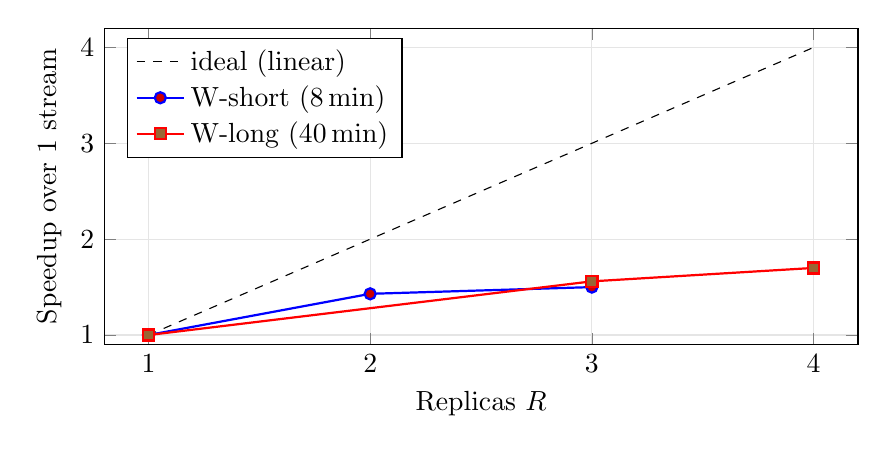
\begin{tikzpicture}
\begin{axis}[
    width=0.92\linewidth, height=5.6cm,
    xlabel={Replicas $R$}, ylabel={Speedup over 1 stream},
    xmin=0.8, xmax=4.2, ymin=0.9, ymax=4.2,
    xtick={1,2,3,4}, legend pos=north west,
    legend cell align=left, grid=both, grid style={gray!20},
]
\addplot[dashed,black,domain=1:4]{x};
\addlegendentry{ideal (linear)}
\addplot+[mark=*,thick,blue,error bars/.cd,y dir=both,y explicit]
  coordinates {(1,1.00) +- (0,0.00) (2,1.43) +- (0,0.001)
               (3,1.50) +- (0,0.003)};
\addlegendentry{W-short (8\,min)}
\addplot+[mark=square*,thick,red,error bars/.cd,y dir=both,y explicit]
  coordinates {(1,1.00) +- (0,0.00) (3,1.56) +- (0,0.00)
               (4,1.70) +- (0,0.009)};
\addlegendentry{W-long (40\,min)}
\end{axis}
\end{tikzpicture}
\caption{Process replicas deliver real but sub-linear speedup, flattening as the
GPU saturates. Error bars are sample SD ($n=5$) and can be smaller than the
markers. Thread-level parallelism (not shown) sits \emph{below} $1.0$.}
\label{fig:speedup}
\end{figure}

\begin{figure}[t]
\centering
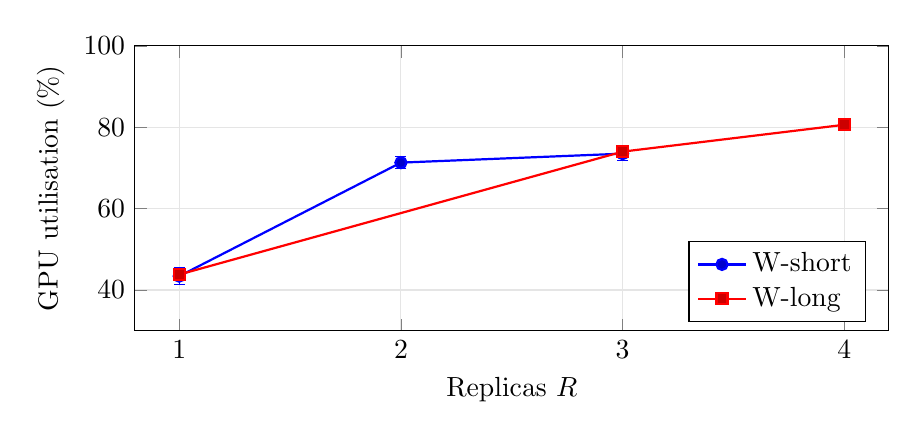
\begin{tikzpicture}
\begin{axis}[
    width=0.92\linewidth, height=5.2cm,
    xlabel={Replicas $R$}, ylabel={GPU utilisation (\%)},
    xmin=0.8, xmax=4.2, ymin=30, ymax=100,
    xtick={1,2,3,4}, legend pos=south east,
    legend cell align=left, grid=both, grid style={gray!20},
]
\addplot+[mark=*,thick,blue,error bars/.cd,y dir=both,y explicit]
  coordinates {(1,43.4) +- (0,2.1) (2,71.3) +- (0,1.5)
               (3,73.5) +- (0,1.6)};
\addlegendentry{W-short}
\addplot+[mark=square*,thick,red,error bars/.cd,y dir=both,y explicit]
  coordinates {(1,43.8) +- (0,0.4) (3,74.0) +- (0,0.6)
               (4,80.6) +- (0,0.6)};
\addlegendentry{W-long}
\end{axis}
\end{tikzpicture}
\caption{Utilisation climbs from $<\!50\%$ (single stream) toward saturation as
replicas are added. Error bars are sample SD ($n=5$). The remaining gap on
W-long reflects heavier CPU-bound diarization for 8 speakers.}
\label{fig:util}
\end{figure}

\subsection{No gateway penalty is observed}
Table~\ref{tab:gateway} compares direct client-side round-robin against routing
through the nginx gateway. The gateway distributes submissions evenly and
routes status polls back to the owning replica correctly. Its repeated mean is
$1.2\%$ higher on W-short and $2.2\%$ higher on W-long. We do not interpret a
proxy as accelerating inference; rather, the positive differences expose
temporal variation between the unpaired direct and gateway series. The data show
no observable throughput penalty, although this descriptive experiment is not
an equivalence test.

\begin{table}[t]
\centering
\caption{Gateway vs.\ direct client-side round-robin, three replicas. Values
are throughput mean (sample SD), $n=5$; difference is
$(T_{\mathrm{gateway}}-T_{\mathrm{direct}})/T_{\mathrm{direct}}$.}
\label{tab:gateway}
\begin{tabular}{lccc}
\toprule
Workload & Direct & Gateway & Difference \\
 & (\filesmin) & (\filesmin) & \\
\midrule
W-short & \msd{8.89}{0.02} & \msd{8.99}{0.43} & $+1.2\%$ \\
W-long  & \msd{1.54}{<0.01} & \msd{1.57}{0.01} & $+2.2\%$ \\
\bottomrule
\end{tabular}
\end{table}

% ===========================================================================
\subsection{A conservative predictive batch model}
\label{sec:model}
For a batch of $N$ homogeneous files on $R$ replicas, each serving one job at a
time, let
\begin{equation*}
  q=\lfloor N/R\rfloor, \qquad r=N\bmod R,
\end{equation*}
so a synchronized schedule contains $q$ full waves and, when $r>0$, one partial
wave. Let $s_j$ denote the representative server-side service time with $j$
concurrently active replicas; for homogeneous jobs with equal completion times,
this is also the wave duration. We estimate $s_j$ by the repeated mean
running$\rightarrow$finished time. If only the full-wave time $s_R$ is
available, a simple estimate is
\begin{equation}
  W_{\mathrm{coarse}} \;\approx\; \lceil N/R\rceil\,s_R,
  \label{eq:model}
\end{equation}
which conservatively charges a partial wave at the full-wave time when reduced
concurrency does not increase service time. When the partial-wave time $s_r$ is
known, the remainder-aware estimate is
\begin{equation}
  W \;\approx\;
  \begin{cases}
    q\,s_R,       & r=0,\\
    q\,s_R+s_r,   & r>0.
  \end{cases}
  \label{eq:model2}
\end{equation}
The earlier single-stream correction is therefore the special case $r=1$, not
a formula for every partial wave.

\paragraph{Validation at small $N$.} Before the end-to-end test we check
Eq.~\eqref{eq:model2} where repetition is cheap enough to bound it tightly:
a \emph{fixed} two-replica deployment ($R{=}2$) with the offered job count
varied from one to four, five repetitions each (Table~\ref{tab:oversub}). This
is the case a deployment actually faces --- the replica count is chosen at
provisioning time and the arrival rate is not.

The model's central prediction is that throughput is \emph{not} monotonic in
$N$. Throughput rises from $N{=}1$ to $N{=}2$, falls at $N{=}3$, and returns at
$N{=}4$ to a value statistically indistinguishable from $N{=}2$: the 95\%
intervals $[8.372, 8.392]$ and $[8.304, 8.416]$ overlap. Contention alone
cannot produce this, since it degrades monotonically; quantisation can, because
a partial wave occupies a full wave's elapsed time while completing fewer jobs,
so $N/W$ peaks whenever $R \mid N$. Quantitatively, the measured $s_1 =
10.18$\,s and $s_2 = 14.31$\,s give predictions of $24.49$\,s at $N{=}3$ and
$28.63$\,s at $N{=}4$, against observed $24.15$\,s and $28.71$\,s --- errors of
$-1.4\%$ and $+0.3\%$ with no fitted parameter.

\begin{table}[t]
\centering
\caption{Eq.~\eqref{eq:model2} at small $N$ on a fixed two-replica deployment
(W-short). Throughput is mean (sample SD) with a two-sided 95\% $t$ interval,
$n=5$. Throughput at $N{=}4$ recovers to the $N{=}2$ value because both are
integer multiples of the replica count; $N{=}3$ pays for a partial wave.}
\label{tab:oversub}
\begin{tabular}{ccccc}
\toprule
Jobs & Throughput & 95\% CI & Predicted $W$ & Observed $W$ \\
$N$ & (\filesmin) & (\filesmin) & (s) & (s) \\
\midrule
1 & \msd{5.896}{0.005} & $[5.889,\,5.903]$ & ---     & $10.18$ \\
2 & \msd{8.382}{0.008} & $[8.372,\,8.392]$ & ---     & $14.31$ \\
3 & \msd{7.462}{0.313} & $[7.073,\,7.851]$ & $24.49$ & $24.15$ \\
4 & \msd{8.360}{0.045} & $[8.304,\,8.416]$ & $28.63$ & $28.71$ \\
\bottomrule
\end{tabular}
\end{table}

The operational reading is that a deployment serving an in-flight count not
divisible by $R$ wastes most of a wave: provisioning should match $R$ to the
expected concurrency, or admit work in multiples of $R$. Adding a replica that
leaves $R \nmid N$ can measurably reduce throughput.

We test Eq.~\eqref{eq:model2} end-to-end by submitting $N{=}10$ identical files
through the gateway with $R{=}3$, so $q=3$ and $r=1$. For W-short, the repeated
means $s_3=17.94$\,s and $s_1=8.70$\,s predict $62.5$\,s; three batches
complete in \msd{60.0}{2.3}\,s. For W-long, $s_3=111.76$\,s and
$s_1=59.76$\,s predict $395.0$\,s; the repeated batch mean is
\msd{370.9}{15.0}\,s (Table~\ref{tab:batch}). The prediction uncertainty in
the table propagates the sample SDs of $s_3$ and $s_1$ under independence; it
does not include model-form uncertainty.

The negative signed errors show a systematic conservative bias, larger than the
input-time variability. The wave model assumes synchronized boundaries and
stationary service times. In a continuously queued batch, however, a replica
starts its next job as soon as it finishes; small completion differences then
stagger ASR, alignment, and diarization across replicas, smoothing resource use
and shortening later service times.

The small-$N$ sweep supplies direct evidence for that mechanism. $N{=}3$ is the
only level in Table~\ref{tab:oversub} whose repetitions are not tightly
clustered: its coefficient of variation is $4.2\%$ against $\le 0.5\%$
elsewhere, and its five wall times fall into two groups --- $22.4$\,s once and
$24.5$--$24.7$\,s four times --- rather than scattering about a mean. $N{=}3$
is also the only level with a partial wave. Under synchronized boundaries the
trailing job would begin only once both replicas had drained, giving
$24.49$\,s; the faster group is what is expected when it instead begins as soon
as the \emph{first} replica frees, overlapping the tail of the other. The
bimodality is thus the same staggering that makes
Equation~\eqref{eq:model2} conservative on the $N{=}10$ batches, observed at a
scale small enough to see individual waves. It also means the $N{=}3$ mean
describes a state the system does not occupy, which is why
Table~\ref{tab:oversub} reports dispersion alongside it. We report the effect
without claiming to have characterised its dependence on replica completion
order.

Equation~\eqref{eq:model2} is therefore a
simple planning estimate, not an exact queueing model. A tighter predictor would
need steady-state, stage-aware service measurements or a discrete-event model.
For a fixed $R$, $s_R$ alone still supports the coarse estimate; the refined
estimate additionally requires $s_r$ for the batch's remainder.

\begin{table}[t]
\centering
\caption{End-to-end batch test through the gateway
(Eq.~\eqref{eq:model2}). Predicted and measured times are mean (sample SD);
$n=5$ for input service times and $n=3$ for batches. Error is
$(W_{\mathrm{meas}}-W_{\mathrm{pred}})/W_{\mathrm{pred}}$.}
\label{tab:batch}
\begin{tabular}{lccc}
\toprule
Batch & Predicted & Measured & Error \\
\midrule
$10\times$ W-short (8\,min)  & \msd{62.5}{0.5}\,s
                                      & \msd{60.0}{2.3}\,s  & $-4.0\%$ \\
$10\times$ W-long (40\,min)  & \msd{395.0}{2.0}\,s
                                      & \msd{370.9}{15.0}\,s & $-6.1\%$ \\
\bottomrule
\end{tabular}
\end{table}

\subsection{Contention is concentrated in ASR and diarisation}
\label{sec:stages}

Per-stage instrumentation (\S\ref{sec:setup}) localises where concurrency is
paid for. Table~\ref{tab:stages} gives the mean duration of each stage at each
offered concurrency.

\begin{table}[t]
\centering
\caption{Server stage means in seconds (share of \texttt{pipeline}), fixed
two-replica deployment, $n=5$ per level. Alignment is invariant to concurrency;
transcription and diarisation roughly double from $c=1$ to $c=2$. Model
preparation is $0.00$ throughout: the caches are mounted and the run is warmed,
so it is excluded by construction.}
\label{tab:stages}
\begin{tabular}{lcccc}
\toprule
Stage & $c=1$ & $c=2$ & $c=3$ & $c=4$ \\
\midrule
Queue wait        & $0.00$ & $0.00$ & $4.44$ & $6.61$ \\
Audio load        & $0.14$ & $0.15$ & $0.15$ & $0.13$ \\
Transcription     & $1.88$ & $3.47$ & $2.91$ & $3.46$ \\
Alignment         & $3.02$ & $2.99$ & $3.04$ & $2.99$ \\
Diarisation       & $3.20$ & $6.26$ & $5.26$ & $6.25$ \\
Speaker assign.   & $0.47$ & $0.47$ & $0.47$ & $0.47$ \\
\midrule
Pipeline total    & $8.72$ & $13.34$ & $11.84$ & $13.30$ \\
\bottomrule
\end{tabular}
\end{table}

Going from one in-flight job to two, transcription grows $1.88 \to 3.47$\,s and
diarisation $3.20 \to 6.26$\,s --- both close to a factor of two, meaning the
two replicas obtain almost no overlap in these stages. Alignment is flat
($3.02 \to 2.99$\,s): it overlaps essentially perfectly. Speaker assignment and
audio load are invariant and negligible.

This is the mechanism behind the $71.1\%$ efficiency at $c=2$. Two of the three
substantial stages serialise on GPU compute while the third does not, so the
achievable speedup is bounded well below linear no matter how many replicas are
added to one GPU. It also identifies diarisation --- $47\%$ of pipeline time at
$c=2$, the single largest component --- as the highest-value target for
optimisation, ahead of the ASR pass that dominates the popular understanding of
transcription cost.

\subsection{Provisioning: the host CPU binds before the GPU}
\label{sec:capacity}

Table~\ref{tab:capacity} reports the marginal resource cost of one concurrent
job, measured as a delta over an idle baseline taken immediately before the
sweep.

\begin{table}[t]
\centering
\caption{Marginal cost of one concurrent job and the resulting ceiling on this
host (12 vCPU, $165.1$\,GiB RAM, one $97\,887$\,MiB GPU). GPU memory is
\emph{incremental}: the idle baseline already holds $18\,625$\,MiB of resident
model weights.}
\label{tab:capacity}
\begin{tabular}{lcc}
\toprule
Resource & Per concurrent job & Host ceiling (jobs) \\
\midrule
CPU           & $2.39$ cores   & $\approx 5$ \\
GPU memory    & $3760$\,MiB    & $\approx 26$ \\
Host RAM      & $0.09$\,GiB    & $\approx 1833$ \\
\bottomrule
\end{tabular}
\end{table}

The binding resource is the host CPU, not the GPU. Twelve vCPUs are exhausted
at roughly five concurrent jobs, while the $96$\,GiB GPU would accommodate
about twenty-six. For a pipeline whose cost is usually discussed in terms of
GPU capability, the accelerator is the abundant resource here and the host is
scarce: a deployment that provisions by GPU memory will be CPU-starved long
before the card is full.

Throughput saturates earlier still, at $c=2$ (\S\ref{sec:model}), so neither
ceiling is reached in practice on this pipeline --- the operative limit is GPU
compute contention. The ceilings nonetheless bound what additional GPUs can
buy: at $2.39$ cores per job, twelve vCPUs cannot feed many more concurrent
jobs regardless of how many accelerators are added, so scaling this deployment
across GPUs requires scaling host cores with them.

Energy is modest: $213$\,W mean draw at the $c=2$ operating point, or
$\approx 3$\,Wh per hour of audio transcribed.

\section{Discussion}
\label{sec:discussion}

\paragraph{When are threads acceptable?} Thread-level workers would help only if
the pipeline released the GIL for (almost) its entire duration. A pure-GPU model
with a thin Python wrapper can approach that; a pipeline with neural diarization
and Python-side clustering does not. The diagnostic is simple and general: if
throughput fails to rise---or utilisation falls---as intra-process concurrency
increases, the workload is GIL/CPU-bound and needs processes, not threads.

\paragraph{How many replicas?} The ceiling is set by GPU compute, not memory:
each replica added utilisation until $\approx 73$--$81\%$, after which per-job
service time lengthened and returns diminished. Three replicas maximised useful
throughput on our single GPU. The heavier, 8-speaker W-long workload saturated at
slightly lower utilisation, consistent with a larger CPU-bound diarization
fraction. Scaling beyond $\approx 1.7\times$ requires additional GPUs, over which
the same replica-plus-gateway design extends directly.

\paragraph{Extrapolation to multiple GPUs.}
The architecture scales across GPUs without modification. Each replica is pinned
to a GPU (via \texttt{CUDA\_VISIBLE\_DEVICES}), and the single gateway
round-robins across \emph{all} replicas irrespective of which GPU hosts them; the
job-id prefix routing (\S\ref{sec:gateway}) is unchanged. With $G$ GPUs and $k$
replicas per GPU the deployment is $R=Gk$ replicas behind one endpoint. Crucially
the workload is \emph{embarrassingly parallel}: each job runs entirely on one
replica and one GPU, with no model sharding and no inter-GPU communication, so
the GPUs do not contend and throughput scales linearly,
\begin{equation}
  T(G) \;\approx\; G \cdot T_1,
  \label{eq:gpuscale}
\end{equation}
where $T_1$ is the measured single-GPU sustained throughput. For $G$ GPUs with
$k$ replicas each, the batch model uses $R=Gk$ in
Eqs.~\eqref{eq:model}--\eqref{eq:model2}; adding GPUs reduces the number of full
waves, while the last wave is priced according to the concurrency actually
assigned to each GPU.

Table~\ref{tab:multigpu} extrapolates to $G=4$ GPUs at the measured sweet spot
$k=3$ ($R=12$ replicas). A batch of ten 40-minute recordings falls from four
nominal waves (\msd{370.9}{15.0}\,s measured) on one GPU to a single wave
($\approx 112$\,s) on four, and sustained long-file throughput rises from $92$
to $\approx 370$ recordings per
hour. The one caveat is that linear scaling holds only while the \emph{shared}
resources keep pace: the gateway (CPU-light) and the \texttt{/data} volume
(disk I/O, negligible beside transcription) are not the concern, but host CPU is.
Because diarization is CPU-bound, each replica consumes host cores, so $R=Gk$
concurrent replicas demand proportional host CPU; on a machine that cannot feed
all $Gk$ replicas the CPU---not the GPUs---becomes the ceiling, and $k$ should be
lowered accordingly. GPU memory is not a constraint ($\approx 13$\,GB per
replica).

\begin{table}[t]
\centering
\caption{Extrapolation to four GPUs at $k=3$ replicas per GPU. Single-GPU
columns are measured; four-GPU columns assume the linear scaling of
Eq.~\eqref{eq:gpuscale} across independent GPUs (subject to the host-CPU caveat).}
\label{tab:multigpu}
\begin{tabular}{lcc}
\toprule
 & 1 GPU (meas.) & 4 GPUs (extrap.) \\
\midrule
Replicas $R=Gk$                       & $3$    & $12$ \\
Throughput, W-short (\filesmin)       & $8.89$ & $35.6$ \\
Throughput, W-long (\filesmin)        & $1.54$ & $6.2$ \\
W-long recordings\,/\,hour            & $92$   & $370$ \\
$10\times$W-short batch (wall)        & \msd{60.0}{2.3}\,s & $\approx 18$\,s \\
$10\times$W-long batch (wall)         & \msd{370.9}{15.0}\,s & $\approx 112$\,s \\
Waves for $N{=}10$                    & $4$    & $1$ \\
\bottomrule
\end{tabular}
\end{table}

\paragraph{Threats to validity.} We study one GPU, one pipeline, and two
recordings; absolute numbers will differ elsewhere. Repeating the same recording
quantifies execution variability, not variability across a population of audio,
languages, speaker counts, or acoustic conditions. Five trials per primary
configuration and three per batch are enough to expose unstable one-off values
but too few for strong distributional assumptions or an equivalence test.
An unrelated model on the other GPU shares host CPU, memory, and I/O resources;
we leave that realistic background service in place and report within-session
sample SD rather than claiming a noise-free machine. Finally, the batch model
assumes homogeneous files, stationary concurrency-specific service times, and
synchronized waves. The repeated batches expose a $4$--$7\%$ conservative bias
when queued jobs desynchronize. Heterogeneous batches require per-file,
stage-aware estimates or a queueing simulation rather than the simple wave sum.

% ===========================================================================
\section{Related Work}
\label{sec:related}

Whisper~\cite{radford2023whisper} and WhisperX~\cite{bain2023whisperx}
established accurate long-form, time-aligned transcription; pyannote provides the
diarization stage~\cite{bredin2020pyannote,bredin2023pyannote,plaquet2023powerset}.
Efficient
inference backends such as CTranslate2~\cite{ctranslate2} accelerate the ASR
step but do not address pipeline-level concurrency. The limitations of the
CPython GIL for multi-threaded compute are long known~\cite{cpythongil}; recent
work on removing it (PEP~703) targets exactly the class of Python-bound
parallelism we observe, and would in principle let the thread-level design
compete with replication. Our contribution is not a new model or runtime but an
empirical characterisation of an inference \emph{service}'s concurrency, the
identification of the process-local registry problem for horizontally replicated
stateful inference, and an empirically evaluated sizing model---practical
guidance that, to
our knowledge, is not documented for this now-ubiquitous pipeline.

% ===========================================================================
\section{Conclusion}
\label{sec:conclusion}

Speaker-attributed transcription is not the GPU-bound workload it appears to be.
On a single GPU we showed that a lone stream wastes half the device, that
thread-level workers regress throughput because the pipeline is GIL/CPU-bound,
and that process-level replication behind a lightweight gateway recovers the
idle capacity---$1.50\times$ at three replicas for W-short and $1.70\times$ at
four for W-long---with no observed proxy penalty. A remainder-aware wave model
provides a conservative batch estimate, overpredicting the repeated ten-file
means by $4$--$7\%$. The recipe is deliberately
mundane: replicate the
process, encode replica identity in the job id, round-robin at a gateway, and
stop adding replicas when the GPU saturates. Because jobs never cross a GPU, the
same design scales out linearly---an estimated $4\times$ on four GPUs
(Table~\ref{tab:multigpu})---until host CPU, not the GPUs, becomes the bound. We
hope it saves other practitioners the detour through thread-level parallelism
that motivated this study.

% ===========================================================================
\appendix
\section{Reproducing the Measurements}
\label{app:repro}

All experiments are driven by the cluster manager and load generator in the
accompanying repository (\url{https://github.com/gtoscano/Parascribe}).
The cluster manager, \path{whisperx_cluster.py}, manages the replicas and
gateway. The load generator, \path{benchmark_transcribe.py}, submits
\texttt{-{}-levels} concurrent jobs per level, warms the models with
\texttt{-{}-warmup}, samples \texttt{nvidia-smi} at 2\,Hz, and writes a CSV whose
throughput and utilisation columns feed the tables. Each invocation below is
annotated with the result it produces. After one warm-up per service
configuration, we run each thread, process, and gateway command five times and
each ten-file batch command three times, changing only the
\texttt{-{}-out} suffix (for example,
\path{measurements/repetitions/process_short_r1.csv}). Our deployment
places the nginx gateway
on port~8357 and the direct replica ports at 8360--8362 (8363 for a fourth
replica); adjust paths and ports for your setup.

\subsection{Cluster setup}
\begin{lstlisting}[language=]
# Pre-download the weights. Only the libraries are baked into the image, so
# without this the first request of a fresh deployment pays the download.
python3 fetch_models.py
python3 fetch_models.py --check   # exits non-zero if anything is missing

# Build the image and start k replicas on one GPU behind the nginx gateway
REPLICAS=3 python3 whisperx_cluster.py up

# Multiple GPUs (Table 6): k replicas PER GPU, interleaved across --gpus.
# 3 x 4 = 12 replicas behind the same single gateway endpoint:
python3 whisperx_cluster.py up --replicas 3 --gpus 0,1,2,3

# Print the direct per-replica URLs (used by the pool experiments)
python3 whisperx_cluster.py urls --direct
#  -> http://localhost:8360,http://localhost:8361,http://localhost:8362
\end{lstlisting}

\subsection{Thread-level parallelism (Table~\ref{tab:threads})}
This experiment uses the single-container service with \texttt{WORKERS=2} fixed
(not the replica cluster). The load
generator varies offered concurrency from one to four jobs: at level~1 only one
worker is active, at level~2 both worker threads are active, and at level~4 the
two workers process the jobs in two waves.
\begin{lstlisting}[language=]
# Set `- WORKERS=2` in docker-compose.yml, then:
docker compose -p whisperx-cluster up -d --build

python3 benchmark_transcribe.py \
    --url http://localhost:8357 \
    --levels 1,2,4 --num-speakers 4 \
    --out paper/measurements/repetitions/thread_short_r1.csv
\end{lstlisting}

\subsection{Process-replica scaling
(Table~\ref{tab:replicas}, Figures~\ref{fig:speedup}--\ref{fig:util})}
Direct client-side round-robin across the replica URLs isolates per-replica
scaling (it bypasses the gateway).
\begin{lstlisting}[language=]
# W-short (8-min AMI, 4 speakers), 1..3 replicas via the sweep
python3 benchmark_transcribe.py \
    --urls http://localhost:8360,http://localhost:8361,http://localhost:8362 \
    --audio testing_audio/dataset/ami/ES2005a.wav \
    --levels 1,2,3 --num-speakers 4 \
    --out paper/measurements/repetitions/process_short_r1.csv

# W-long (40-min Oyez, 8 speakers), three replicas
python3 benchmark_transcribe.py \
    --urls http://localhost:8360,http://localhost:8361,http://localhost:8362 \
    --audio testing_audio/dataset/oyez/2000.99-1978-t01.wav \
    --levels 1,3 --num-speakers 8 \
    --out paper/measurements/repetitions/process_long_3rep_r1.csv

# W-long, four replicas (REPLICAS=4 python3 whisperx_cluster.py up first)
python3 benchmark_transcribe.py \
    --urls http://localhost:8360,http://localhost:8361,\
http://localhost:8362,http://localhost:8363 \
    --audio testing_audio/dataset/oyez/2000.99-1978-t01.wav \
    --levels 4 --num-speakers 8 \
    --out paper/measurements/repetitions/process_long_4rep_r1.csv
\end{lstlisting}

\subsection{Gateway comparison and batch test
(Tables~\ref{tab:gateway}--\ref{tab:batch})}
Point the load generator at the single gateway URL; nginx distributes submissions
and routes status polls back to the owning replica by the job-id prefix. The
gateway rows of Table~\ref{tab:gateway} are the \texttt{-{}-url} runs at
concurrency~3; the direct rows are the \texttt{-{}-urls} runs above at the
matching concurrency.
\begin{lstlisting}[language=]
# W-short gateway comparison (repeat five times)
python3 benchmark_transcribe.py \
    --url http://localhost:8357 \
    --levels 3 --num-speakers 4 \
    --out paper/measurements/repetitions/gateway_short_r1.csv

# W-long gateway comparison (repeat five times)
python3 benchmark_transcribe.py \
    --url http://localhost:8357 \
    --audio testing_audio/dataset/oyez/2000.99-1978-t01.wav \
    --levels 3 --num-speakers 8 \
    --out paper/measurements/repetitions/gateway_long_r1.csv

# Ten-file batches (repeat each three times)
python3 benchmark_transcribe.py \
    --url http://localhost:8357 \
    --audio testing_audio/dataset/ami/ES2005a.wav \
    --levels 10 --num-speakers 4 \
    --out paper/measurements/repetitions/batch_short_r1.csv

python3 benchmark_transcribe.py \
    --url http://localhost:8357 \
    --audio testing_audio/dataset/oyez/2000.99-1978-t01.wav \
    --levels 10 --num-speakers 8 \
    --out paper/measurements/repetitions/batch_long_r1.csv
\end{lstlisting}

% ===========================================================================
\begin{thebibliography}{9}

\bibitem{radford2023whisper}
A.~Radford, J.~W.~Kim, T.~Xu, G.~Brockman, C.~McLeavey, and I.~Sutskever,
``Robust Speech Recognition via Large-Scale Weak Supervision,''
\emph{Proc. ICML}, 2023. arXiv:2212.04356.

\bibitem{bain2023whisperx}
M.~Bain, J.~Huh, T.~Han, and A.~Zisserman,
``WhisperX: Time-Accurate Speech Transcription of Long-Form Audio,''
\emph{Proc. Interspeech}, 2023. arXiv:2303.00747.

\bibitem{baevski2020wav2vec2}
A.~Baevski, H.~Zhou, A.~Mohamed, and M.~Auli,
``wav2vec 2.0: A Framework for Self-Supervised Learning of Speech
Representations,'' \emph{Proc. NeurIPS}, 2020. arXiv:2006.11477.

\bibitem{bredin2020pyannote}
H.~Bredin \emph{et al.},
``pyannote.audio: neural building blocks for speaker diarization,''
\emph{Proc. ICASSP}, 2020.

\bibitem{bredin2023pyannote}
H.~Bredin,
``pyannote.audio 2.1 speaker diarization pipeline: principle, benchmark, and
recipe,'' \emph{Proc. Interspeech}, 2023.

\bibitem{plaquet2023powerset}
A.~Plaquet and H.~Bredin,
``Powerset multi-class cross entropy loss for neural speaker diarization,''
\emph{Proc. Interspeech}, 2023. (Basis of the \texttt{pyannote/segmentation-3.0}
and \texttt{speaker-diarization-3.1} pipelines used here.)

\bibitem{paszke2019pytorch}
A.~Paszke \emph{et al.},
``PyTorch: An Imperative Style, High-Performance Deep Learning Library,''
\emph{Proc. NeurIPS}, 2019.

\bibitem{ctranslate2}
OpenNMT, ``CTranslate2: Fast inference engine for Transformer models,''
\url{https://github.com/OpenNMT/CTranslate2}, 2024.

\bibitem{fasterwhisper}
SYSTRAN, ``faster-whisper: Faster Whisper transcription with CTranslate2,''
\url{https://github.com/SYSTRAN/faster-whisper}, 2024.

\bibitem{cpythongil}
Python Software Foundation, ``The Python Global Interpreter Lock,'' CPython
documentation and PEP~703 (Making the GIL optional),
\url{https://peps.python.org/pep-0703/}.

\bibitem{carletta2005ami}
J.~Carletta \emph{et al.},
``The AMI Meeting Corpus: A Pre-Announcement,''
\emph{Proc. MLMI}, 2005.

\end{thebibliography}

\end{document}
